% !TEX TS-program = pdflatex
% !TEX encoding = UTF-8 Unicode

% This is a simple template for a LaTeX document using the "article" class.
% See "book", "report", "letter" for other types of document.

\documentclass[11pt]{article} % use larger type; default would be 10pt

\usepackage[utf8]{inputenc} % set input encoding (not needed with XeLaTeX)

%%% PAGE DIMENSIONS
\usepackage{geometry}
\geometry{a4paper}
% \geometry{margin=2in} % for example, change the margins to 2 inches all round
% \geometry{landscape} % set up the page for landscape
%   read geometry.pdf for detailed page layout information

\usepackage{graphicx}
\graphicspath{{./images/}}
\usepackage[parfill]{parskip} % Activate to begin paragraphs with an empty line rather than an indent

%%% PACKAGES
\usepackage{booktabs} % for much better looking tables
\usepackage{array} % for better arrays (eg matrices) in maths
\usepackage{paralist} % very flexible & customizable lists (eg. enumerate/itemize, etc.)
\usepackage{verbatim} % adds environment for commenting out blocks of text & for better verbatim
\usepackage{subfig} % make it possible to include more than one captioned figure/table in a single float

%%% HEADERS & FOOTERS
\usepackage{fancyhdr} % This should be set AFTER setting up the page geometry
\pagestyle{fancy} % options: empty , plain , fancy
\renewcommand{\headrulewidth}{0pt} % customize the layout...
\lhead{}\chead{}\rhead{}
\lfoot{}\cfoot{\thepage}\rfoot{}

%%% SECTION TITLE APPEARANCE
\usepackage{sectsty}
\allsectionsfont{\sffamily\mdseries\upshape}

%%% ToC (table of contents) APPEARANCE
\usepackage[nottoc,notlof,notlot]{tocbibind} % Put the bibliography in the ToC
\usepackage[titles,subfigure]{tocloft} % Alter the style of the Table of Contents
\renewcommand{\cftsecfont}{\rmfamily\mdseries\upshape}
\renewcommand{\cftsecpagefont}{\rmfamily\mdseries\upshape} % No bold!

\title{Survival Analysis with Apache Spark and Apache SystemML on Stackexchange}
\author{Mateo Álvarez Calvo}
%\date{} % Activate to display a given date or no date (if empty),
         % otherwise the current date is printed

\newcolumntype{C}[1]{>{\centering\arraybackslash}m{#1}}   %% centered
\newcolumntype{R}[1]{>{\raggedleft\arraybackslash}m{#1}}  %% right aligned



\begin{document}

\maketitle

\newpage
\tableofcontents
\newpage

\section{Introduction \& main goals}
  \label{sec:introduction}
  Many studies have been done over the Stackexchange community [such as], one of the biggest Q\&A sites in the world. The present is yet another study over the data of the famous site, but in this case, the study has two particularities, the use of Apache Spark with the library of Apache SystemML for the processing in a parallel environment, and the use of Survival Analysis to analyze the impact of the variables in the time an answer is accepted for each question, the "survival of each question" in the community.


  \subsection{Main technologies}

    As one of the biggest Q\&A communities, Stackexchange has large amount of data of each interaction.
    Stackexchange is separated in several communities, regarding different topics. These communities can be small, as [] or really big, as Stackoverflow, the developers community. This particularity makes necessary the use of technologies prepared to process large amounts of data, in the later case.

    The purpose of the present study is to analyze this big community, so a distributed processing technology has to be used. For this purpose, Apache Spark, the latest distributed open-source processing technology, has been chosen to parallelize the operations on the data.

    Spark ML is the machine learning library of spark, which contains lots of algorithms. It also includes some Survival Analysis algorithms, but just for parametric modeling. This gives an excuse to use the recently adopted by the Apache Foundation SystemML, a machine learning library developed by IBM, which has non, semi and parametric algorithms for survival analysis.

    Regarding the development environment, Jupyter Notebook provides a simple and flexible interface for this analysis, and can also be integrated with Spark, allowing the complete development in just one environment.

  \subsubsection{Apache Spark}

    Apache Spark is a distributed processing technology developed in Scala by Databricks that represents the next step of Apache Hadoop, including the best parts of it, such as the Hadoop File System, but under a complete new paradigm that allows operations different from the famous map-reduce, using RAM as storage for results rather than writing to disk, lazy and optimized execution of tasks, and special focus on machine learning and SQL-like language, to mention some of the main features.

  \subsubsection{Apache SystemML}

    Recently included in the Apache Foundation Incubating  program, Apache SystemML is a machine learning library that works over distributed frameworks, Spark or Hadoop, written in Java.

    This library provides many distributed implementations of important algorithms as well as a sintaxis to create new algorithms in a distributed mode. It provides a high-level declarative machine learning language, which has two variations, the R-like sintaxis, DML, and the Python-like sintaxis, Py-DML. These self made algorithms pass through a compilation process and are optimized for a distributed environment.

    It can be executed in a variety of distributed and non distributed modes, with it's standalone mode, and the integration with Hadoop, and Spark via SystemML context, which allows the interaction through Scala, Python and R.


  \subsection{The Stackexchange data}
  \label{subsec:data_structure}

    \subsubsection{Stack Exchange}

    Stack Exchange is a network of Q\&A websites created in 2009 after the great success the creators obtained with \emph{Stack Overflow} community in 2008, a Q\&A community website for computer programming.

    Each community covers a different topic, from physics to software, and is structured in a reputation award format. Each site has questions, answers and users, all subjected to this reputation award process.

    All these communities generate large amounts of data, data thet Stackexchange facilitates every once in a while for data scientists and people in general to download and analyze. The data is available in a torrent file and each package has about 35 - 40 GB of compressed information.

    This compressed file has data from different communities for a certain period of time. In this case, the analysis is done over the Scifi community, which is a median size community for science-fiction Q\&A.

    \subsubsection{Scifi community}

    Scifi is a community in Stack Exchange that focuses on science fiction and fantasy. This community was selected because it has a medium size which is perfect to test the mentioned technologies in a reasonable period of time. Selecting just the data from Scifi community from the big compressed file, it weights around 110 MB in a 7z compressed format. This allows the computation on a local machine for experimentation and then scale the problem to a bigger community such as \emph{Ask Ubuntu} or \emph{Stack Overflow} when the process is refined and it can be launched remotely in a cluster, as the data structure is common to al other communities. The data is divided in 8 files, regarding different information:

    \begin{table}[!h]
      \centering
      \begin{tabular}{|c|p{0.3\textwidth}|c|}
        \hline

        File & Description & Size \\ \hline
        Votes.xml & Voting results for each question and more cosas & 84,1 MB \\ \hline
        Tags.xml & Relational table for tags on each question & 169 KB \\ \hline
        Users.xml & Users on the net & 16,7 MB \\ \hline
        PostLinks.xml & links to posts & 1,5 MB \\ \hline
        Posts.xml & List of all questions & 137,3 MB \\ \hline
        PostHistory.xml & All interactions of each post & 268,6 MB \\ \hline
        Comments.xml & List of all comments of each post & 66,3 MB \\ \hline
        Badges.xml & All users' badges & 16,1 MB \\

        \hline
      \end{tabular}
      \caption{List of files from the compressed Scifi folder}
      \label{tab:list_of_files}
    \end{table}

    Further details about the relational database structure is explained below, the objective is to show the variables obtained from the dataset so that the later variable selection is understood.

    \subsubsection{Votes.xml}

      This file contains information about votes of the users to each question. The file has the following structure:

      \begin{table}[!h]
        \centering
        \begin{tabular}{|c|c|p{0.3\textwidth}|}
          \hline
          Feature & Data type & Description \\ \hline
          Id & Integer & Unique vote identifier \\ \hline
          PostId & Integer & Foreign key that indicates the post that was voted \\ \hline
          VoteTypeId & Integer & Type of vote, 1 for Downvote and 2 for Upvote \\ \hline
          CreationDate & Timestamp YYYY-MM-DDTHH:MM:SS.dScSmS & Time of votation \\ \hline
        \end{tabular}
        \caption{Votes table}
        \label{tab:votes}
      \end{table}

    \subsubsection{Tags.xml}

      This file contains all tags and the posts that contains them. The file has the following structure:

      \begin{table}[!h]
        \centering
        \begin{tabular}{|c|c|p{0.3\textwidth}|}
          \hline

          Feature & Data type & Description \\ \hline
          Id & Integer & Unique tag identifier \\ \hline
          TagName & Text & Name of the tag \\ \hline
          Count & Integer & Number of times used \\ \hline
          ExcerptPostId & Integer & \\ \hline
          WikiPostId & Integer & \\

          \hline
        \end{tabular}
        \caption{Tags table}
        \label{tab:tags}
      \end{table}
\newpage
    \subsubsection{Users.xml}

      This file contains information about users. The file has the following structure:

      \begin{table}[!h]
        \begin{tabular}{|c|p{0.3\textwidth}|p{0.35\textwidth}|}
          \hline

          Feature & Data type & Description \\ \hline
          Id & Integer & Unique user identifier \\
          Reputation & Integer & Reputation level of the user \\ \hline
          CreationDate & Timestamp YYYY-MM-DDTHH:MM:SS.dScSmS & User creation date \\ \hline
          DisplayName & Text & Alias to display on question \\ \hline
          LastAccessDate & Timestamp YYYY-MM-DDTHH:MM:SS.dScSmS & Last login date \\ \hline
          WebsiteUrl & Text & Site where the user signed up to \\ \hline
          Location & Text & Location of the user \\ \hline
          AboutMe & Text & Information user provided \\ \hline
          Views & Integer & User views count \\ \hline
          UpVotes & Integer & User up votes count \\ \hline
          DownVotes & Integer & User down votes count \\ \hline
          AccountIf & Integer & Unique user identifier \\

          \hline
        \end{tabular}
        \caption{Users table}
        \label{tab:users}
      \end{table}

    \subsubsection{PostLinks.xml}

      This file contains information about relation between posts. The file has the following structure:

      \begin{table}[!h]
        \begin{tabular}{|c|p{0.3\textwidth}|p{0.35\textwidth}|}
          \hline

          Feature & Data type & Description \\ \hline
          Id & Integer & Unique post links identifier \\
          CreationDate & Timestamp YYYY-MM-DDTHH:MM:SS.dScSmS & Post links creation date \\ \hline
          PostId & Integer & Post unique identifier \\ \hline
          RelatedPostId & Integer & Unique identifier of the post related to the PostId \\ \hline
          LinkTypeId & Integer & Type of relation between posts \\

          \hline
        \end{tabular}
        \caption{Post links table}
        \label{tab:postlinks}
      \end{table}

    \subsubsection{Posts.xml}

      This file contains all questions posted along with the accepted answers and other info related to the time and user who posted the question. The file has the following structure:

      \begin{table}[!h]
        \centering
        \begin{tabular}{|c|p{0.3\textwidth}|p{0.35\textwidth}|}
          \hline

          Feature & Data type & Description \\ \hline
          Id & Integer & Unique question identifier \\ \hline
          PostTypeId & Integer & Type of post codified as integer \\ \hline
          CreationDate & Timestamp YYYY-MM-DDTHH:MM:SS.dScSmS & Time of question creation in extended format \\ \hline
          Score & Integer & Question's score, calculated from the users' votes \\ \hline
          ViewCount & Integer & Count of all visualizations of the question \\ \hline
          Body & Text & The question itself, in utf8 format \\ \hline
          OwnerUserId & Integer & Id of the user who posted the question \\ \hline
          LastEditorUserId & Integer & \\ \hline
          LastEditDate & Timestamp YYYY-MM-DDTHH:MM:SS.dScSmS & Last edition date \\ \hline
          LastActivityDate & Timestamp YYYY-MM-DDTHH:MM:SS.dScSmS & Last interaction with the question time \\ \hline
          Title & Text & Title of the question \\ \hline
          Tags & Text & Tags added to the question \\ \hline
          AnswerCount & Integer & Number of answers to the question \\ \hline
          CommentCount & Integer & Number of comments to the question posted \\ \hline
          FavoriteCount & Integer & Number of times the question has been added to favorite by another user \\ \hline
          ClosedDate & Timestamp YYYY-MM-DDTHH:MM:SS.dScSmS & Time the question has been closed \\ \hline
          CommunityOwnedDate & Timestamp YYYY-MM-DDTHH:MM:SS.dScSmS & Time \\

          \hline
        \end{tabular}
        \caption{Posts table}
        \label{tab:posts}
      \end{table}

    \subsubsection{PostHistory.xml}

      This file contains information about the interactions with each post. The file has the following structure:

      \begin{table}[!h]
        \centering
        \begin{tabular}{|c|p{0.3\textwidth}|p{0.35\textwidth}|}
          \hline

          Feature & Data type & Description \\ \hline
          Id & Integer & Unique interaction identifier \\ \hline
          PostHistoryTypeId & Integer & Type of interaction with the post () \\ \hline
          PostId & Integer & Unique identifier of the post this interaction is related to \\ \hline
          RevisionGUID & Text &  \\ \hline
          CreationDate & Timestamp YYYY-MM-DDTHH:MM:SS.dScSmS & Time of question creation in extended format \\ \hline
          UserId & Integer & Unique identifier of the user that created the interaction with the post \\ \hline
          Text & Text & Text the user introduced on the interaction \\ \hline

          \hline
        \end{tabular}
        \caption{Post history table}
        \label{tab:posthistory}
      \end{table}

    \subsubsection{Comments.xml}

      This file contains the comments posted for every question created. The file has the following structure:

      \begin{table}[!h]
        \centering
        \begin{tabular}{|c|p{0.3\textwidth}|p{0.35\textwidth}|}
          \hline

          Feature & Data type & Description \\ \hline
          Id & Integer & Unique comment identifier \\ \hline
          PostId & Integer & Unique identifier of the post this comment is related to \\ \hline
          Score & Integer & Total score of the comment \\ \hline
          Text & Text & Comment text \\ \hline
          CreationDate & Timestamp YYYY-MM-DDTHH:MM:SS.dScSmS & Time of comment creation in extended format \\ \hline
          UserId & Integer & Unique identifier of the user who posted the comment \\

          \hline
        \end{tabular}
        \caption{Comments table}
        \label{tab:comments}
      \end{table}

    \subsubsection{Badges.xml}

      This file contains information about the badges the user has obtained.

      \begin{table}[!h]
        \centering
        \begin{tabular}{|c|p{0.3\textwidth}|p{0.35\textwidth}|}
          \hline

          Feature & Data type & Description \\ \hline
          Id & Integer & Unique Badge identifier \\ \hline
          UserId & Integer & Unique identifier of the user who obtained the badge \\ \hline
          Name & Text & Name of the badge \\ \hline
          Date & Timestamp YYYY-MM-DDTHH:MM:SS.dScSmS & Time the user obtained the badge in extended format \\ \hline
          Class & Integer & Type of the badge \\ \hline
          TagBased & Boolean & Whether the badge is based on a tag or not \\

          \hline
        \end{tabular}
        \caption{Comments table}
        \label{tab:badges}
      \end{table}

  \subsection{Main Objectives}

    The main objective of this study is to test the scalability and integration of the proposed technologies, Spark, SystemML and Jupyter Notebook in the usecase of Stack Exchange communities, so further data analysis can be performed. This main goal is divided in three major goals:

    \begin{itemize}

      \item Use Spark to make the data cleaning to create a script for further research on the Stackexchange site.

      \item Verify SystemML integration with Spark for further research and scalability.

      \item Use SystemML survival analysis algorithms to analyze Stackexchange's data and obtain conclusions on the main variables affecting the time taken by the community to answer each question.

    \end{itemize}

\newpage

\section{Technologies}
  \label{sec:technologies}

  The downloaded data from Stackexchange for the analysis weights about 40 GB, which is enough amount to consider distributed processing. Going down to the distributed processing frameworks, Apache Spark was chosen

  \subsection{Apache Spark}

    Apache Spark is a fast and general-purpose cluster computing system, widely used for data processing. It provides high-level APIs in Java, Scala, Python and R, and an optimized engine that supports general execution graphs. It also supports a rich set of higher-level tools including Spark SQL for SQL and structured data processing, MLlib and SparkML for machine learning and pipelines, GraphX for graph processing, and Spark Streaming.

    This distributed data processing framework was initially developed at the University of California, Berkeley's AMPLab, and donated to the Apache Software Foundation in February 2014, the first release was on May 30th 2014.

    Apache Hadoop presented some limitations that Apache Spark tried to solve:

    \begin{itemize}
      \item It is difficult to write most of the algorithms in a MapReduce form.
      \item It is very slow to write each iteration to disk, which, for example makes difficult to use Hadoop to process streaming.
      \item Apache Hadoop's support for iterative jobs and Machine Learning restricts it's use for this task.
      \item Apache Hadoop's SQL tools doesn't work well on complex queries, sometimes it doesn't work at all and other times it is quite slow as it writes on HDD each iteration.
    \end{itemize}

    Some solutions Apache Spark provides to these problems are:

    \begin{itemize}
      \item Lazy computation, Spark only executes a set of tasks when a result is required. This gives the opportunity to optimize jobs before executing them.
      \item In-memory data caching, Spark scans HDD only once to read the input data and then uses RAM as much as it can, which is faster than scanning disk on every step.
      \item
    \end{itemize}

    \subsubsection{Spark Data Structure}




    \subsubsection{Apache Spark Structure}

      Spark has a master-slave architecture and supports various resource managers: standalone, Mesos and YARN. The resource manager will only be in charge of identify the resources. Independently of the resource manager chosen, the Apache Spark architecture doesn't change.

      All Spark processes share the same architecture, the driver process takes care of calculating the job's parallelism and calculates every job's stage. Each stage is divided on a series of tasks, which will be sent to the executors, where will be executed. The communication between the Spark application and the resource manager will be done through a SparkContext.

      The deployment of Spark has two variants, client and cluster mode. On the client mode, the Driver is launched on the machine the process has been invoked, and it can be inside or outside the cluster. On cluster mode, the cluster manager is assigned to control the Driver process, and the process itself will be launched inside the cluster. In case Mesos is the cluster manager, it will require an additional service.[][][][][][][]

      Apache Spark is formed by the Spark Core API, available in R, SQL, Python, Scala and Java languages, and built up on it four main libraries: Spark SQL + DataFrames, Spark Streaming, Spark MLlib, Spark ML and GraphX, that complements functionality for Spark, specially on the parts Hadoop failed, Machine Learning, SQL and Streaming.



      \subsubsection*{Spark Core API}

        The core API represents the basic structure of Spark, it can be addressed form any of the supported languages, scala, python, R and java.

      \subsubsection*{Spark SQL + DataFrames}

        The SQL layer over data is known as Spark SQL

      \subsubsection*{Spark MLlib + Spark ML}

        Spark has two main Machine Learning libraries, the first one, Spark MLlib, which is the basic library, that includes the main algorithms and is addressed with RDDs, the second one, Spark ML, which uses Spark MLlib but through DataFrames, and includes further functionality, such as Pipelines, a set of operations performed over data, that allows the user to build sequences of actions over Data Frames.

      \subsubsection*{Spark GraphX}

        GraphX is Spark's graph library, which is used to interact with graphs.





  \subsection{Apache SystemML}

    Developed by IBM, Apache SystemML is the [precursor] of Spark ML (MLLib), the machine learning libraries of Spark.
    SystemML is coded in a self-made programming language, Distributed Machine Learning (DML) and it can be used from Spark or Hadoop in a [submit-like execution or in a interactive execution, the one it has been used in this study].

    SystemML has a high level API which can be addressed from Python-like or R-like sintaxis, and then transformed to the low level DML (Distributed Machine Learning) language.

    \subsubsection{SystemML Structure}



  \subsection{Reproducible research with Python, Scala and Jupyter}

    Regarding the selection of the development environment, it was important to use a standardized one so that the analysis could be reproduced by anyone. Jupyter notebook is one of the most commonly used, specially in the education and investigation institutions. Jupyter Notebook is easy to use and configure and it can be easily integrated with Spark. It has interactive interpreters for many languages, including python, ruby, scala, R, etc

    To configure the same environment as the one used in this study, some steps have to be followed:

    \subsubsection{Environment setup}

      The versions of the software used for this study are listed below:

    \begin{table}[!h]
      \centering
      \begin{tabular}{| c | c |}
        \hline

        Technology & Version \\ \hline
        Jupyter Notebook & 4.3.1 \\ \hline
        Python & 3.5 \\ \hline
        Scala & 2.11 \\ \hline
        Toree kernel & 0.2.0.dev1 \\ \hline
        Spark & 2.1 \\ \hline
        SystemML & 0.12.0 \\

        \hline
      \end{tabular}
      \caption{Technologies and versions used}
    \end{table}

    The first step is to setup Jupyter Notebook, either running it in a Docker container or installing it directly on the machine. The docker image can be obtained entering the following command in a shell: \emph{docker pull jupyter/notebook}. Regarding the other option, installing it, the instructions can be found in the following link: \emph{http://jupyter.readthedocs.io/en/latest/install.html}.

    Once Jupyter Notebook is running, the kernels have to be configured. In this study, Scala and Python were used for the data processing, so both kernels were configured. The python kernel is usually configured, as it comes with the IPython kernel installation, if not, follow the guide[][][][][]. To install the scala kernel, several options can be considered, as there are several implementations of the scala kernel. The chosen one was Scala Toree.

    Apart from the kernels, some dependencies must be installed to do the data processing in python, those dependencies are:

    \begin{itemize}
      \item appnope==0.1.0
      \item bokeh==0.12.4
      \item botocore==1.5.43
      \item findspark==1.1.0
      \item ipykernel==4.5.2
      \item ipython==5.3.0
      \item ipython-genutils==0.1.0
      \item matplotlib==2.0.0
      \item notebook==4.3.1
      \item numpy==1.12.0
      \item pandas==0.19.2
      \item py4j==0.10.4
      \item pyparsing==2.2.0
      \item python-dateutil==2.6.0
      \item scipy==0.18.1
      \item systemml==0.14.0
      \item toree==0.2.0.dev1
      \item traitlets==4.3.2
    \end{itemize}

    For the python kernel, the SystemML library has to be installed, instructions for the installation can be found in the Apache SystemML's get started documentation: https://systemml.apache.org/install-systemml.html


\section{Infrastructure and resources}
  \label{sec:infrastructure_and_resources}

  As commented before, selecting an environment to be used is the first step, and it is a essential part.

  \subsection{Architecture scheme}

    The whole study has been executed in a standalone model, with a MacBookPro Retina 2015. The data was stored in an HDFS

  \subsection{Configuration}



  \subsection{Workflow}

    The first step is to clean the data and make the feature selection. One the data is clean, it is used as the input for the models training, both Kaplan-Meier model and Cox Proportional Hazards Model.

  \subsubsection{Data cleaning}
    The data provided by StackOverflow comes in a reasonably clean xml set of files, which were previously described, on section \ref{subsec:data_structure}.




\section{Results}
  \label{sec:results}

  \subsection{Survival Analysis}

    Survival analysis is a set of different techniques and algorithms used to estimate the time passed until the occurrence of an event. All of these methods are based on the conditional probability of an event occurring in a certain period of time, usually called \emph{Hazard Rate}. This basic idea can be applied to numerous environments, such as time of failure of a component in the industry, time of occurrence of an event in economics, and others, but the main field of application of these methodologies is the medical, where the time until some event is usually important.

    As in every statistic methodology, there are dependent and independent variables, usually called covariates. In this case, the dependent variable is, as mentioned before, the hazard rate, the conditional probability of an event occurring in a certain period of time, but the analysis is not only restricted to assess the effect of the covariates in the time to an event, but also the impact of these variables on the hazard rate.

      Among the collection of methods included under Survival Analysis, two have special interest for different reasons, these two models are introduced here and explained in detail below.

    The first one is the Kaplan-Meier model, which is a simple, Non-parametric model used for simple and fast analysis, and the representation of the survivor curve. This method in particular, along with the \emph{Life Table} are classic methods useful for a fast but imprecise analysis of the data. Kaplan-Meier's use is more extended although it is more suitable for small samples.

    On the other hand, Cox Proportional-hazards regression is a more complex model, introduced in 1972 by Sir David Cox, in the paper \emph{Regression Models and Life Tables}, which is nowadays one of the 100 most important papers in all of science, as it introduces key innovations in the field.

  \subsection{Used data}

    The data used for the analysis has already been presented on section \ref{subsec:data_structure}, so the point of view of this section is to present the input data format necessary for the \emph{Survival Analysis} methods and how has the study's data transformed for it.

    \subsubsection{Data censoring and truncation}

      Data censoring refers to a situation where some data of the instance is known but some event times are not known, for example when the event occurs after the end of the observation period. Data truncation refers to the lack of information of some variables outside of the time period considered in the study.

      \begin{figure}
        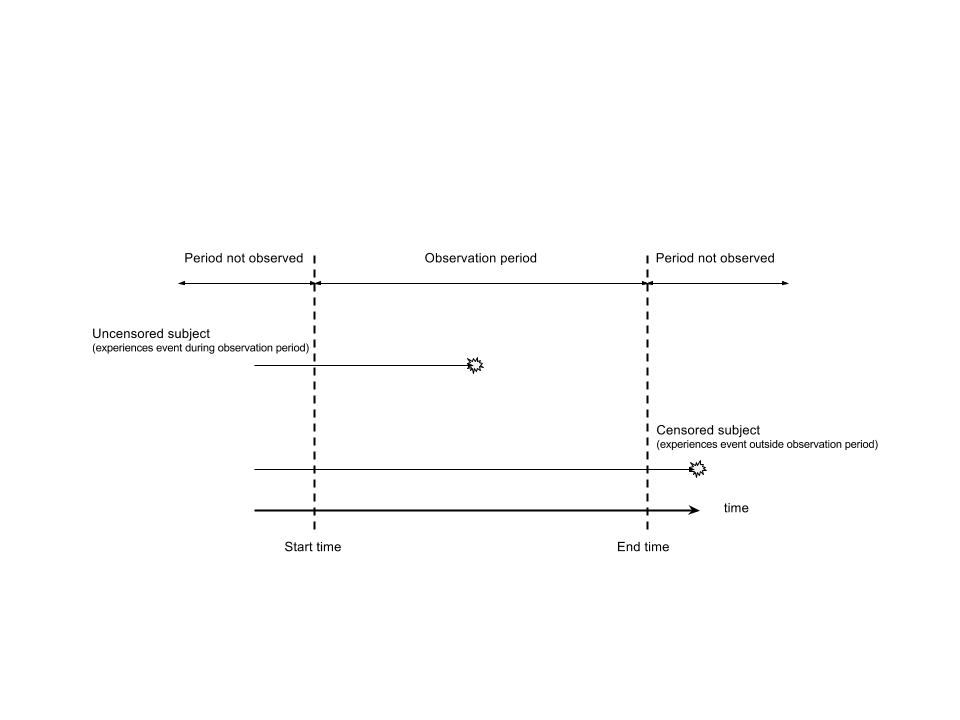
\includegraphics[width=\textwidth]{Data_censoring.png}
        \caption{Censored and uncensored data}
        \label{img:data_censoring}
      \end{figure}

      There are different situations of data censoring,

    \subsubsection{Data structure}


  \subsection{Kaplan-Meier model}



  \subsection{Cox Proportional Hazards Model}

\section{Conclusions}
  \label{sec:conclusions}

  \subsection{Most important results}

  \subsection{Lessons learnt}



\end{document}
